\appendix
%% Правка оформления ссылок на приложения:
%http://tex.stackexchange.com/questions/56839/chaptername-is-used-even-for-appendix-chapters-in-toc
%http://tex.stackexchange.com/questions/59349/table-of-contents-with-chapter-and-appendix
%% требует двойной компиляции
\addtocontents{toc}{\def\protect\cftchappresnum{\appendixname{} }%
\setlength{\cftchapnumwidth}{\widthof{\cftchapfont\appendixname~Ш\cftchapaftersnum}}%
}
%% Оформление заголовков приложений ближе к ГОСТ:
\sectionformat{\chapter}[display]{% Параметры заголовков разделов в тексте
    label=\chaptertitlename\ \thechapter,% (ГОСТ Р 2.105, 4.3.6)
    labelsep=20pt,
}
\renewcommand\thechapter{\Asbuk{chapter}} % Чтобы приложения русскими буквами нумеровались

%=======================
%======APPENDIX A=======
%=======================
\chapter{Интерфейсная модель} \label{AppendixA}

Интерфейсная модель содержит классы и интерфейсы для взаимодействия с пользователем.

\begin{figure} [h] 
  \center
  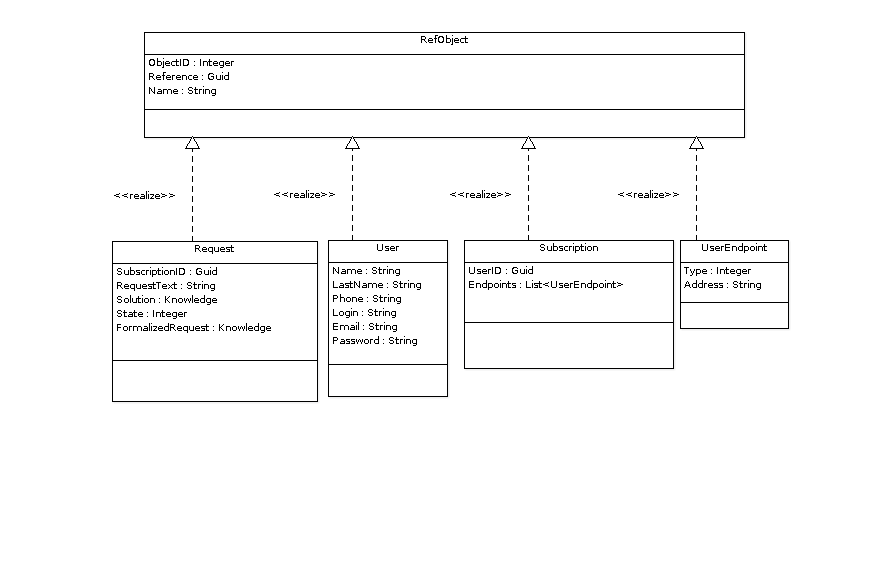
\includegraphics [scale=0.8,angle=90, origin=c] {interface-model}
  \caption{Диаграмма классов интерфейсной модели} 
  \label{img:interface-model}  
\end{figure}

\emph{RefObject}

Представляет собой общий объект, который сохраняется в Базе Знаний. (Базовый класс для всех остальных классов и объектов)
\begin{itemize}
	\item ObjectID- уникальный в пределах класса ключ
	\item Reference- уникальный в пределах всех баз знаний ключ
	\item Name-имя объекта
\end{itemize}

\emph{Request}

Объект для хранения запроса пользователя.
\begin{itemize}
	\item SubscriptionID - идентификатор подписки
	\item RequestText - запрос пользователя в виде текста
	\item Solution - ссылка на решение запроса
	\item State - статус запроса (например, Поиск Решения)
	\item FormalizedRequest - ссылка на формализованный запрос
\end{itemize}


\emph{Subscription}

Информация о подписке пользователя на события
\begin{itemize}
	\item Endpoints - списко UserEndpoint, которые будут использоваться для обратной связи с пользователем
\end{itemize}

\emph{UserEndpoint}
\begin{itemize}
	\item Type - тип точки связи с пользователем (например, веб-сервис)
	\item Address - адрес точки связи с пользователем
\end{itemize}
\clearpage

%=======================
%======APPENDIX B=======
%=======================
\chapter{Описание модуля Action} \label{AppendixB}
Action является базовым классом для WayToThink или Critic.
\begin{figure} [h] 
  \center
  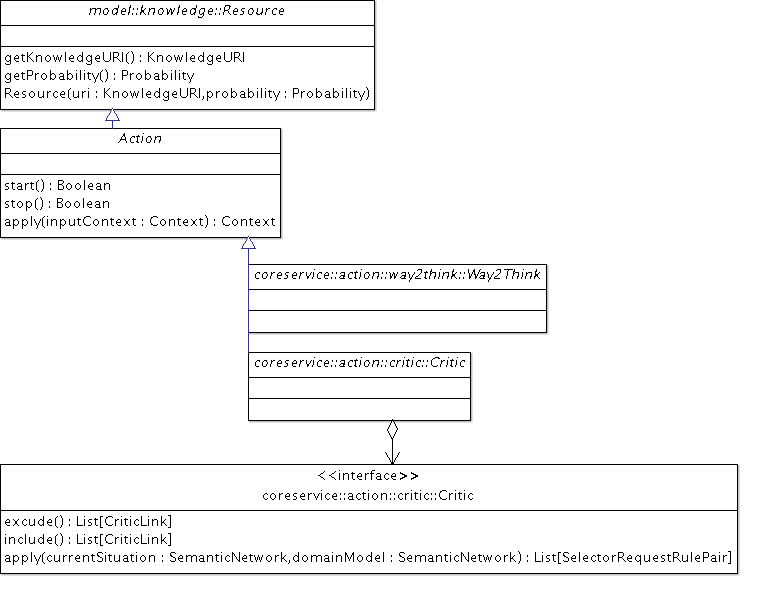
\includegraphics [scale=0.6, origin=c] {ActionClass}
  \caption{Диаграмма классов Action} 
  \label{img:ActionClass}  
\end{figure}

\clearpage
%=======================
%======APPENDIX C=======
%=======================
\chapter{Описание модуля Цели} \label{AppendixC}
Goal (Цель) является набором вероятностных предикатов и последовательностью How-To необходимых для того, чтобы достичь цель. Goal и How-To тесно связаны. На Рисунке \ref{img:goal} показан состав Goal. Goal состоит из:
\begin{enumerate}
	\item Parameters - параметры, которые используются предикатами для выполнения
	\item Precondition - условия, которые должны быть выполнены до выполнения проверок цели
	\item Entry criteria - входной критерий, предикат, который определяет, что цель активировалась
	\item Exite criteria - условия, когда цель считается выполненной
	\item PostCondition - дополнительные условия для выхода
	\item HowTo - набор решения. Список путей решения
\end{enumerate}

\begin{figure} [h] 
  \center
  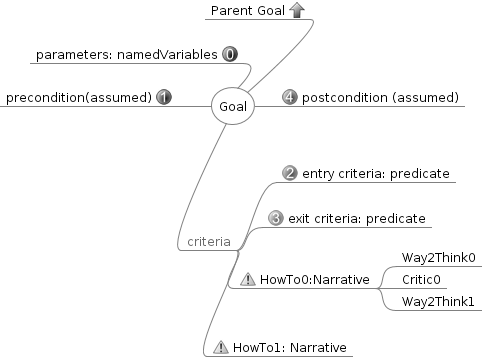
\includegraphics [scale=1.0, origin=c] {goal}
  \caption{Диаграмма классов Goal} 
  \label{img:goal}  
\end{figure}

\textbf{Типы предикатов} \\
В решение используется 3 типа логических предикатов: and, or, not. Представление Goal в SemanticNetwork показано на диаграмме \ref{img:2_0_GoalHowToConcept}.

\begin{figure} [h] 
  \center
  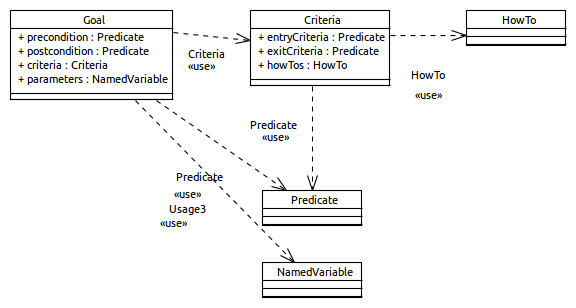
\includegraphics [scale=1.0, origin=c] {2_0_GoalHowToConcept}
  \caption{Диаграмма места Goal в SemanticNetwork (Семантической сети)} 
  \label{img:2_0_GoalHowToConcept}  
\end{figure}

Иерархия целей имеет высшую цель: Помочь пользователю. Далее вниз по иерархии идут подцели: Решить инцидент, Понять тип инцидента, Найти решение инцидента и т.д.

\clearpage
%=======================
%======APPENDIX D=======
%=======================
\chapter{Рецепты решений} \label{AppendixDHowTo}
Рецепты решений представляют собой последовательность действий выполняемых для решения проблемы, описанной в инциденте. 
Было разработано два типа HowTo: ValueHowTo-содержит в себе простое значение; FunctionalHowTo- содержит в себе функцию. \\
FunctionalHowTo состоит из следующих частей:
\begin{enumerate}
	\item FunctionalBody - тело функции, описывающий содержание функции
	\item InputParameters - входные параметры функции
	\item OutputParameters - выходные параметры
\end{enumerate}
Комбинация FunctionaHowTo и ValueHowTo является Рецептом Решения. Например, решение проблемы неработающего сегмента кластера в формате для специалиста технической поддержки.
\begin{itemize}
	\item Войти на сервер U1
	\item Запустить утилиту 12 для Windows Servers
	\item Открыть вкладку 1
	\item Перейти на All Managed Server, найти нужный Server из правой панели, открыть свойства сервера
	\item Нажать на Backup Exec Services
	\item Выберите проблемный сегмент кластера
	\item Нажмите Restart all Services
	\item Подождите и проверьте статус
\end{itemize}
Преобразованный в формат HowTo данный рецепт решения будет выглядеть как показано ниже.
\clearpage
\begin{lstlisting}
	login:howto{
  Parameters:[

    {Key:'ScriptName',
    Value:'LogonScript.bat'},
    {Key:'Description',
    Value:'Logon to server'}
  ]

  InputParameters:[
    {Key:'ServerName',
    Value:'U1'},
    {Key:'UserName',
    Value:'MyUser'}
  ]

  OutputParameters:[
    {Key:'SessionID',
    Value:'SSSE12'},

  ]
}

launch:howto{
  Parameters:[

    {Key:'ScriptName',
    Value:'LaunchScript.bat'},
    {Key:'Description',
    Value:'Launch the application'}
  ]

  InputParameters:[
    {Key:'ExecName',
    Value:'Utility12.exe'},
  ]

  OutputParameters:[
    {Key:'SessionID',
    Value:'SSSE12'},

  ]
}
\end{lstlisting}
%=======================
%======APPENDIX E=======
%=======================
\clearpage
\chapter{Экспериментальные данные}\label{AppendixE}
Часть экспериментальных данных (Общая длина файла примерно 10000 инцидентов).
\begin{lstlisting}
	

EUROPE DOMAIN NEW SERVER Request Form
*(M)* unable to connect remotely to other machine 
Quota limit on the personal file store exceeded Europemuk176 
TCP/IP Address Management Request 
Quota limit exceeded 
EUROPED007 caiW2kOs:w2kLVolInst C: is now Critical at 03:16:10
EUROPEM116 caiW2kOs:w2kProcInst DRWTSN32,*,* is now Critical at 11:51:03
2011-04-29 20:16:50 EUROPEM239 LogWatcher BABBACKUP 2011-04-30 06:05:55 EUROPEMUK212 LogWatcher NetBDBMgr File SYSTEM_LOG 
EUROPEMUK521 WinA3_NetInst:InErrors Intel[R] 82567LF-3 Gigabit Network \\ Connection is now Warning at 
EUROPEMUK521 WinA3_NetInst:InErrors Intel[R] 82567LF-3 Gigabit Network Connection is now Critical a \\
CSDTS02 The NSM/TNG NT4 System Agent reports Logical Volume C: has reached CRITICAL utilisation at \\
CSDTS02 The NSM/TNG NT4 System Agent reports Logical Volume D: has reached CRITICAL utilisation at \\
EUROPEMUK521 WinA3_NetInst:InErrors Intel[R] 82567LF-3 Gigabit Network Connection is now Warning at \\
CSAPP01 Possible hardware problem detected - Please investigate with HP Insight Manager \\
CSAPP02 Possible hardware problem detected - Please investigate with HP Insight Manager \\
EUROPEMUK521 WinA3_NetInst:InErrors Intel[R] 82567LF-3 Gigabit Network Connection is now Warning at \\
EUROPEMUK521 WinA3_NetInst:InErrors Intel[R] 82567LF-3 Gigabit Network Connection is now Warning at\\
EUROPEM218 CA Backup - Backup_Operation_Failed at 23:20, 30/04/11
FMSDTS02 The NSM/TNG Win2k System Agent reports Logical Volume D: has reached CRITICAL utilisation\\
FMSDTS02 The NSM/TNG Win2k System Agent reports Logical Volume D: has reached WARNING state at 23:4\\
EUROPEVUK140 caiW2kOs:w2kMemPhys Physical Memory is now Warning at 00:05:25
2011-05-01 00:27:37 EUROPEMUK236 LogWatcher CA_Backup_F Backup_Operation_Failed File \\
EUROPEMUK521 WinA3_NetInst:InErrors Intel[R] 82567LF-3 Gigabit Network Connection is now Warning at\\
EUROPEMUK521 WinA3_NetInst:InErrors Intel[R] 82567LF-3 Gigabit Network Connection is now Critical a\\
2011-05-01 00:51:37 EUROPEMUK236 LogWatcher CA_Backup_F Backup_Operation_Failed File \\
EUROPEMUK521 WinA3_NetInst:InErrors Intel[R] 82567LF-3 Gigabit Network Connection is now Warning at \\
2011-05-01 01:33:37 EUROPEMUK236 LogWatcher CA_Backup_W Check_Device_Group File \\
EUROPEVUK232 WinA3_CPUTotal:TotalLoad CPUTotal is now Critical at 01:50:42 \\
EUROPEMUK521 WinA3_NetInst:InErrors Intel[R] 82567LF-3 Gigabit Network \\ Connection is now Warning at 
EUROPEMUK521 WinA3_NetInst:InErrors Intel[R] 82567LF-3 Gigabit Network \\ Connection is now Warning at \\
EUROPEMUK521 WinA3_NetInst:InErrors Intel[R] 82567LF-3 Gigabit Network \\ Connection is now Warning at 
FLETCHER The NSM/TNG Win2k System Agent reports Logical Volume C: has reached WARNING state at 02:4 \\
EUROPEMUK521 WinA3_NetInst:InErrors Intel[R] 82567LF-3 Gigabit Network \\ Connection is now Warning at
EUROPEMUK521 WinA3_NetInst:InErrors Intel[R] 82567LF-3 Gigabit Network \\ Connection is now Warning at
EUROPEMUK521 WinA3_NetInst:InErrors Intel[R] 82567LF-3 Gigabit Network \\ Connection is now Warning at
EUROPEMUK521 WinA3_NetInst:InErrors Intel[R] 82567LF-3 Gigabit Network \\ Connection is now Warning at
EUROPEVUK232 WinA3_CPUTotal:TotalLoad CPUTotal is now Warning at 04:56:43 \\ 
EUROPEMUK521 WinA3_NetInst:InErrors Intel[R] 82567LF-3 Gigabit Network \\ Connection is now Warning at
EUROPEMUK521 WinA3_NetInst:InErrors Intel[R] 82567LF-3 Gigabit Network \\ Connection is now Critical a
EUROPEMUK521 WinA3_NetInst Intel[R] 82567LF-3 Gigabit Network Connection is now Critical at 05:40:5 
EUROPEMUK521 WinA3_NetInst:InErrors Intel[R] 82567LF-3 Gigabit Network \\ Connection is now Warning at
EUROPEMUK521 WinA3_NetInst:InErrors Intel[R] 82567LF-3 Gigabit Network \\ Connection is now Warning at
EUROPEMUK521 WinA3_NetInst:InErrors Intel[R] 82567LF-3 Gigabit Network \\ Connection is now Warning at
EUROPEMUK541 caiWinA3 caiWinA3 is now DOWN at 09:46:20 \\
EUROPEMUK521 WinA3_NetInst:InErrors Intel[R] 82567LF-3 Gigabit Network Connection is now Critical a
EUROPEVUK216 caiW2kOs:w2kNetTotal Net Total is now Critical at 11:02:05 \\
EUROPEM218 CA Backup - Backup_Operation_Failed at 11:54, 01/05/11 \\
EUROPEVUK140 caiW2kOs:w2kMemPhys Physical Memory is now Warning at 12:35:25 \\
EUROPEMUK521 WinA3_NetInst:InErrors Intel[R] 82567LF-3 Gigabit Network  \\Connection is now Warning at
EUROPEMUK521 WinA3_NetInst:InErrors Intel[R] 82567LF-3 Gigabit Network \\Connection is now Warning at
EUROPEMUK541 caiLogA2 caiLogA2 is now DOWN at 13:49:20 \\
EUROPEMUK541 caiWinA3 caiWinA3 is now DOWN at 13:49:31 \\
UKM145 caiW2kOs:w2kCpuInst CPU 0 is now Warning at 14:53:24 \\
EUROPEMUK521 WinA3_NetInst:InErrors Intel[R] 82567LF-3 Gigabit Network Connection is now Warning at
EUROPEMUK521 WinA3_NetInst:InErrors Intel[R] 82567LF-3 Gigabit Network \\ Connection is now Warning at
EUROPEMUK521 WinA3_NetInst:InErrors Intel[R] 82567LF-3 Gigabit Network \\ Connection is now Warning at
EUROPEMUK541 caiWinA3 caiWinA3 is now DOWN at 17:47:51 \\
EUROPEMUK521 WinA3_NetInst:InErrors Intel[R] 82567LF-3 Gigabit Network \\Connection is now Warning at
EUROPEVUK232 WinA3_CPUTotal:TotalLoad CPUTotal is now Critical at 18:52:43 \\
EUROPEVUK039 Mib-II:IP_Interface 172.19.12.218 is now Broken at 19:06:42 \\
EUROPEMUK521 WinA3_NetInst:InErrors Intel[R] 82567LF-3 Gigabit Network \\Connection is now Warning at
EUROPEVUK039 caiW2kOs:w2kSrvcInst CASUniversalAgent is now Critical at 19:24:53 \\
EUROPEMUK521 WinA3_NetInst:InErrors Intel[R] 82567LF-3 Gigabit Network \\Connection is now Critical a
EUROPEVUK050A Mib-II:IP_Interface 172.19.244.7 is now Broken at 19:52:07 \\
EDISON Mib-II:IP_Interface 172.19.244.76 is now Broken at 19:54:02 \\
EUROPEVUK053A Mib-II:IP_Interface 172.19.244.8 is now Broken at 19:54:59 \\
EUROPEMUK521 WinA3_NetInst:InErrors Intel[R] 82567LF-3 Gigabit Network \\ Connection is now Warning at
CSDTS02 The NSM/TNG NT4 System Agent reports Logical Volume C: has reached \\ CRITICAL utilisation at
2011-05-01 22:05:36 EUROPEMUK236 LogWatcher CA_Backup_F Unable_To_Find_Any_Media File  \\
2011-05-01 22:05:36 EUROPEMUK236 LogWatcher CA_Backup_F   Backup_Operation_Failed File \\
2011-05-01 22:07:36 EUROPEMUK236 LogWatcher CA_Backup_F Backup_Operation_Failed File \\
EUROPEMUK521 WinA3_NetInst:InErrors Intel[R] 82567LF-3 Gigabit Network Connection is now Warning at \\
CSAPP02 Possible hardware problem detected - Please investigate with HP Insight Manager \\
CSAPP01 Possible hardware problem detected - Please investigate with HP Insight Manager \\
EUROPEVUK232 WinA3_CPUTotal:TotalLoad CPUTotal is now Warning at 00:32:44 \\
EUROPEMUK521 WinA3_NetInst:InErrors Intel[R] 82567LF-3 Gigabit Network \\ Connection is now Warning at
EUROPEMUK521 WinA3_NetInst:InErrors Intel[R] 82567LF-3 Gigabit Network \\ Connection is now Critical a
EUROPEMUK521 WinA3_NetInst:InErrors Intel[R] 82567LF-3 Gigabit Network \\ Connection is now Critical a
EUROPEMUK541 caiWinA3 caiWinA3 is now DOWN at 01:50:22
EUROPEMUK541 caiLogA2 caiLogA2 is now DOWN at 01:50:24 \\
EUROPEMUK521 WinA3_NetInst:InErrors Intel[R] 82567LF-3 Gigabit Network \\ Connection is now Warning at
EUROPEM116 caiW2kOs:w2kCpuInst CPU 0 is now Warning at 03:25:03
EUROPEMUK521 WinA3_NetInst:InErrors Intel[R] 82567LF-3 Gigabit Network \\ Connection is now Warning at
EUROPEMUK521 WinA3_NetInst:InErrors Intel[R] 82567LF-3 Gigabit Network \\ Connection is now Warning at
EDISON Mib-II:IP_Interface 172.19.244.76 is now Broken at 19:54:02 \\
2011-05-02 05:01:47 EUROPEMUK212 LogWatcher NetBDBMgr File SYSTEM_LOGapplication MatchPattern FILE \\
2011-05-02 05:13:47 EUROPEMUK212 LogWatcher NetBDBMgr File SYSTEM_LOGapplication MatchPattern FILE \\
EUROPEM116 caiW2kOs:w2kCpuInst CPU 0 is now Warning at 05:25:03
CSDTS02 The NSM/TNG NT4 System Agent reports Logical Volume C: has reached WARNING state at 05:26, \\
EUROPEMUK521 WinA3_NetInst:InErrors Intel[R] 82567LF-3 Gigabit Network Connection is now Critical a
EUROPEMUK529 WinA3_NetInst:InBytes Intel[R] 82578DM Gigabit Network Connection is now Warning at 05 \\
EUROPEMUK521 WinA3_NetInst Intel[R] 82567LF-3 Gigabit Network Connection is now Critical at 05:40:5 \\
EUROPEMUK541 caiLogA2 caiLogA2 is now DOWN at 05:48:16 \\
EUROPEMUK541 caiWinA3 caiWinA3 is now DOWN at 05:48:52 \\
CSDTS02 The NSM/TNG NT4 System Agent reports Logical Volume C: has reached WARNING state at 06:08, \\
UKM145 caiW2kOs:w2kCpuInst CPU 0 is now Warning at 06:57:22 \\
UKM145 caiW2kOs:w2kCpuInst CPU 1 is now Warning at 06:57:22 \\
2011-05-02 07:01:17 UKM205 LogWatcher BABBACKUP is now Critical \\
2011-05-02 07:39:36 EUROPEMUK236 LogWatcher CA_Backup_I Media_Error File D:Program Files CABright \\
EUROPEVUK053A caiW2kOs:w2kProcInst DRWTSN32,*,* is now Critical at 09:44:01 \\
EUROPEMUK521 WinA3_NetInst:InErrors Intel[R] 82567LF-3 Gigabit Network \\ Connection is now Critical a
EUROPEMUK521 WinA3_NetInst:InErrors Intel[R] 82567LF-3 Gigabit Network \\ Connection is now Warning at
EUROPEMUK521 WinA3_NetInst:InErrors Intel[R] 82567LF-3 Gigabit Network \\ Connection is now Warning at
EDISON Mib-II:IP_Interface 172.19.244.76 is now Broken at 19:54:02 \\
EUROPEMUK521 WinA3_NetInst:InErrors Intel[R] 82567LF-3 Gigabit Network Connection is now Warning at
LUCAS caiW2kOs:w2kCpuInst CPU 0 is now Critical at 14:27:59 \\
LUCAS caiW2kOs:w2kCpuTotal CPU Total is now Critical at 14:27:59 \\
UKM145 caiW2kOs:w2kCpuInst CPU 0 is now Warning at 14:55:21 \\
UKM145 caiW2kOs:w2kCpuInst CPU 1 is now Warning at 14:57:21 \\
2011-05-02 15:01:17 UKM205 LogWatcher BABBACKUP is now Critical \\
2011-05-02 17:01:59 EUROPEMUK268 LogWatcher BABbackup File\\ 
2011-05-02 17:06:50 EUROPEMUK176 LogWatcher BABBACKUP File \\ 
2011-05-02 20:17:01 EUROPEM239 LogWatcher BABBACKUP File \\ 
 caiLogA2 caiLogA2 is now DOWN at 21:48:52 \\
CSDTS02 The NSM/TNG NT4 System Agent reports Logical Volume C: has reached \\ CRITICAL utilisation at
CSAPP01 Possible hardware problem detected - Please investigate with HP  \\ Insight Manager
CSAPP02 Possible hardware problem detected - Please investigate with HP \\ Insight Manager
EUROPEMUK521 WinA3_NetInst:InErrors Intel[R] 82567LF-3 Gigabit Network \\ Connection is now Warning at
EUROPEMUK521 WinA3_NetInst:InErrors Intel[R] 82567LF-3 Gigabit Network \\ Connection is now Critical a
2011-05-02 23:32:02 EUROPEMUK177 LogWatcher BABBACKUP File \\
EUROPEMUK521 WinA3_NetInst:InErrors Intel[R] 82567LF-3 Gigabit Network Connection is now Warning at
2011-05-03 05:01:46 EUROPEMUK212 LogWatcher NetBDBMgr File SYSTEM_LOG\application MatchPattern FILE
2011-05-03 05:13:46 EUROPEMUK212 LogWatcher NetBDBMgr File SYSTEM_LOG\application MatchPattern FILE
EUROPEMUK521 WinA3_NetInst:InErrors Intel[R] 82567LF-3 Gigabit Network Connection is now Warning at
CSDTS02 The NSM/TNG NT4 System Agent reports Logical Volume C: has reached WARNING state at 05:30,
EUROPEMUK521 WinA3_NetInst:InErrors Intel[R] 82567LF-3 Gigabit Network Connection is now Critical a
EUROPEMUK521 WinA3_NetInst Intel[R] 82567LF-3 Gigabit Network Connection is now Critical at 05:40:5
EUROPEMUK541 caiLogA2 caiLogA2 is now DOWN at 05:50:00
EUROPEMUK541 caiWinA3 caiWinA3 is now DOWN at 05:50:08
2011-05-03 06:23:35 EUROPEMUK236 LogWatcher CA_Backup_I Media_Error File D:\Program Files\CA\Bright
2011-05-03 06:31:35 EUROPEMUK236 LogWatcher CA_Backup_I Media_Error File D:\Program Files\CA\Bright
EUROPEMUK521 WinA3_NetInst:InErrors Intel[R] 82567LF-3 Gigabit Network Connection is now Critical a
EUROPEMUK521 WinA3_NetInst:InErrors Intel[R] 82567LF-3 Gigabit Network Connection is now Warning at
FLETCHER The NSM/TNG Win2k System Agent reports Logical Volume C: has reached WARNING state at 07:5
EUROPEMUK521 WinA3_NetInst:InErrors Intel[R] 82567LF-3 Gigabit Network Connection is now Warning at
EUROPEMUK521 WinA3_NetInst:InErrors Intel[R] 82567LF-3 Gigabit Network Connection is now Critical a
EUROPEMUK521 WinA3_NetInst:InErrors Intel[R] 82567LF-3 Gigabit Network Connection is now Critical a
2011-05-03 09:02:02 EUROPEMUK177 LogWatcher BABBACKUP File C:\Program Files\CA\ARCserve Backup\LOG\
 D: drive on Europemde011 is in warning state.
EUROPE DOMAIN NEW SERVER Request Form Submitted via 7799 Web Site
 drive on Europemde011 is in warning state.
EUROPEMUK521 WinA3_NetInst:InErrors Intel[R] 82567LF-3 Gigabit Network Connection is now Warning at
EUROPEMUK521 WinA3_NetInst:InErrors Intel[R] 82567LF-3 Gigabit Network Connection is now Critical a
LUCAS caiW2kOs:w2kCpuInst CPU 0 is now Critical at 14:27:59
LUCAS caiW2kOs:w2kCpuTotal CPU Total is now Critical at 14:27:59
EUROPEMUK521 WinA3_NetInst:InErrors Intel[R] 82567LF-3 Gigabit Network Connection is now Warning at
EUROPE DOMAIN NEW SERVER
EUROPE DOMAIN NEW SERVER
EUROPE DOMAIN NEW SERVER
EUROPEMUK521 WinA3_NetInst:InErrors Intel[R] 82567LF-3 Gigabit Network Connection is now Warning at
EUROPEMUK521 WinA3_NetInst:InErrors Intel[R] 82567LF-3 Gigabit Network Connection is now Warning at
EUROPEMUK521 WinA3_NetInst:InErrors Intel[R] 82567LF-3 Gigabit Network Connection is now Warning at
EUROPEMUK521 WinA3_NetInst:InErrors Intel[R] 82567LF-3 Gigabit Network Connection is now Warning at
EUROPEMUK521 WinA3_NetInst:InErrors Intel[R] 82567LF-3 Gigabit Network Connection is now Warning at
EUROPEMUK521 WinA3_NetInst:InErrors Intel[R] 82567LF-3 Gigabit Network Connection is now Warning at
EUROPEMUK521 WinA3_NetInst:InErrors Intel[R] 82567LF-3 Gigabit Network Connection is now Warning at
EUROPEMUK521 WinA3_NetInst:InErrors Intel[R] 82567LF-3 Gigabit Network Connection is now Warning at
EUROPEMUK521 WinA3_NetInst:InErrors Intel[R] 82567LF-3 Gigabit Network Connection is now Warning at
EUROPEMUK521 WinA3_NetInst:InErrors Intel[R] 82567LF-3 Gigabit Network Connection is now Warning at
EUROPEMUK529 WinA3_NetInst:OutPkts Intel[R] 82578DM Gigabit Network Connection is now Warning at 13
EUROPEMUK529 WinA3_NetInst:OutPkts Intel[R] 82578DM Gigabit Network Connection is now Warning at 13
EUROPEMUK521 WinA3_NetInst:InErrors Intel[R] 82567LF-3 Gigabit Network Connection is now Warning at
EUROPEMUK521 WinA3_NetInst:InErrors Intel[R] 82567LF-3 Gigabit Network Connection is now Warning at
EUROPEVUK083 caiW2kOs:w2kCpuInst CPU 0 is now Critical at 13:25:27
EUROPEMUK521 WinA3_NetInst:InErrors Intel[R] 82567LF-3 Gigabit Network Connection is now Warning at
EUROPEMUK521 WinA3_NetInst:InErrors Intel[R] 82567LF-3 Gigabit Network Connection is now Warning at
2011-05-03 14:26:27 EUROPEM240 LogWatcher BABHOLD File C:\Program Files\CA\ARCserve Backup\LOG\Back
2011-05-03 14:28:02 EUROPEMUK177 LogWatcher BABHOLD File C:\Program Files\CA\ARCserve Backup\LOG\Ba
2011-05-03 14:28:50 EUROPEMUK176 LogWatcher BABHOLD File C:\Program Files\CA\ARCserve Backup\LOG\Ba
2011-05-03 14:30:14 EUROPEMUK178 LogWatcher BABHOLD File C:\Program Files\CA\ARCserve Backup\LOG\Ba
2011-05-03 14:47:47 EUROPEMUK177 LogWatcher BABHOLD is now Critical
2011-05-03 14:56:27 EUROPEM240 LogWatcher BABHOLD File C:\Program Files\CA\ARCserve Backup\LOG\Back
EUROPEMUK521 WinA3_NetInst:InErrors Intel[R] 82567LF-3 Gigabit Network Connection is now Warning at
EUROPEMUK521 WinA3_NetInst:InErrors Intel[R] 82567LF-3 Gigabit Network Connection is now Warning at
EUROPEMUK521 WinA3_NetInst:InErrors Intel[R] 82567LF-3 Gigabit Network Connection is now Warning at
TCP/IP Address Management Request Form
\end{lstlisting}
